\documentclass[serif,11pt]{beamer}
\usetheme{Darmstadt}
\usepackage[spanish]{babel}
\usepackage{graphicx}
\begin{document}

	\title {PuzLive}  
	\author {Leonardo Tamayo\\ Carlos Caicedo \\ Pedro I\~niguez}
	\institute{ Facultad de Ingenie\'ia en Electricidad y Computaci\'on\\
		  ESPOL}
	\date[Octubre, 2012]{Octubre, 2012\\}
	

	\begin{frame}
		\titlepage
	\end{frame}

	\begin{frame}
		\frametitle{Contenido}\tableofcontents
	\end{frame} 


	\section{Introducci\'on} 

		\subsection{Lo que nos ofrece}

			\begin{frame}\frametitle{Funcionalidades}
				\pause
				\bigskip
				 
				\begin{itemize}
					 \bigskip
					\item Juego de Rompecabezas 
					\pause
					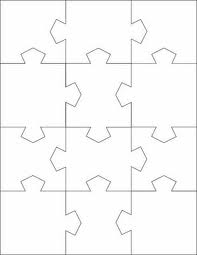
\includegraphics[height=0.1\textwidth]{rompeca} 
					\bigskip
					\pause
					
					\item El sensor de movimiento activa la particion de la imagen y la pantalla tactil es la via para mover las piezas 
					\pause
					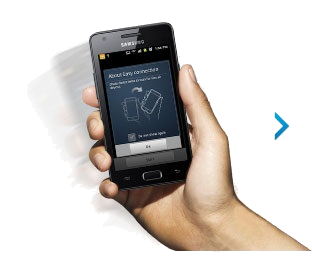
\includegraphics[width=0.1\textwidth]{shake} 
					\bigskip
					\pause
					\item La ilustracion del rompecabezas es la imagen que recibe la camara en cada fotograma
					\bigskip
					\pause
					
\includegraphics[width=0.1\textwidth]{camara1} 
					\bigskip

				\end{itemize}
			\end{frame}

		\subsection{Avances}
		
			\begin{frame}\frametitle{Resumen de Avances}
				\pause \bigskip
				\begin{block}{Resumen de Avances}
					\begin{columns}
						\column{.3\textwidth} \hspace{0.5cm}
						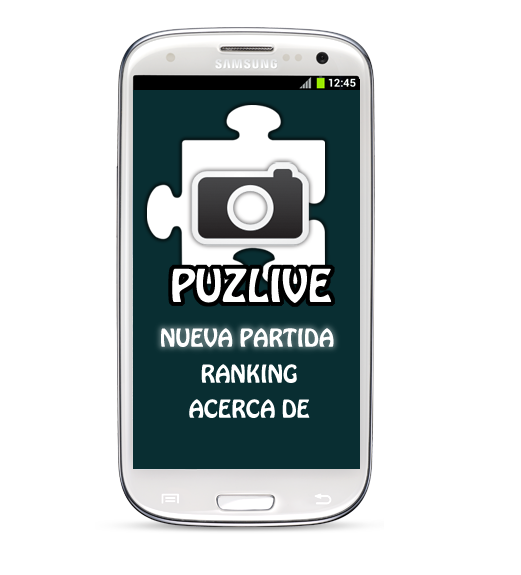
\includegraphics[width=1\textwidth]{androidpro4} 
						\column{.5\textwidth}
						En base a lo anteriormente expuesto, nos propusimos a desarrollar la aplicacion, de
						tal manera que tuviera un menu que mostrara las opciones del juego, tanto la de
						iniciar la partida, ranking, entre otros, mostrar las dificultades y pasar al momento 
						en el que se activa la camara y el video se parte.	
					\end{columns}
				\end{block}
			\end{frame}

		

	\section{Descripci\'on de los Avances} 
		\subsection{Inicializar}


		\begin{frame}
			\frametitle{Icono de Aplicacion}

			\begin{block}{Icono de PuzLive}
					
				La aplicacion cuenta con su propio icono una vez instalado en el dispositivo, para inicializar la aplicaci\'on.
					\begin{itemize}
						 \pause
						\item  
						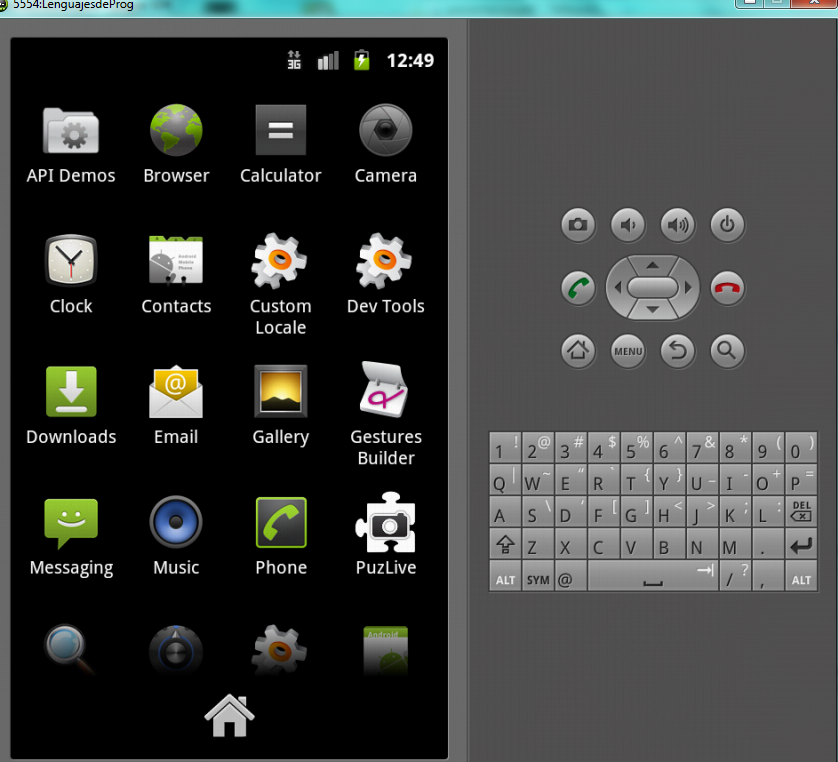
\includegraphics[width=0.5\textwidth]{outmenu} 
						\bigskip
					\end{itemize}
					
				\end{block}
		\end{frame}




		\subsection{Interacci\'on}
		\begin{frame}
			\frametitle{Menu de Inicio}
				\begin{block}{Menu Inicial}
				Se despliega el Menu con las diferentes opciones del programa, al seleccionar "Iniciar Partida" Se despliegan los niveles
				\includegraphics<1>[height=5cm]{menu1} 
				\includegraphics<2>[height=5cm]{puzzle6} 
				\end{block}
		\end{frame}

		
		
		\subsection{Rompecabezas + Video}

		\begin{frame}
			\frametitle{Implementacion de la Camara}
				\begin{block}{Grabando y Partiendo}
					\begin{columns}
						\column{.3\textwidth} \hspace{0.1cm}
						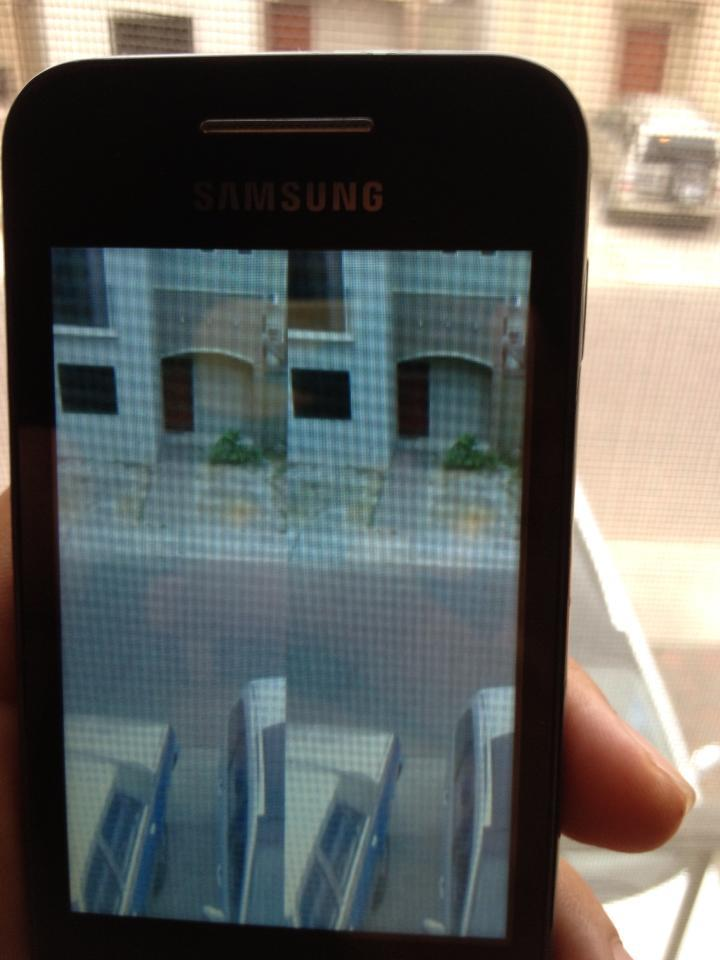
\includegraphics[width=\textwidth]{vidcam} 
						\column{.5\textwidth}

						Se ha logrado activar la camara y partirla de tal manera que se tengan bloques de la misma imagen.
						
						
					\end{columns}
				\end{block}
		\end{frame}


	\subsection{Desarrollo Proximo}
		\begin{frame}
			\frametitle{Aspectos restantes}

			\begin{block}{Lo que esta en proceso de desarrollo}
										
						\begin{itemize}
							 \pause
							\item Activar la particion del rompecabezas con el acelerometro.
							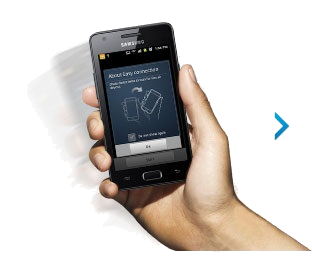
\includegraphics[width=0.1\textwidth]{shake} 
							\bigskip
							\pause
							\item Modificar la matriz IMAGEN y dividirla en pequeñas imagenes.

							\bigskip
							\pause
							\item Desplazar las piezas por medio de la pantalla tactil y evaluar su ubicacion con respecto a la Imagen real
							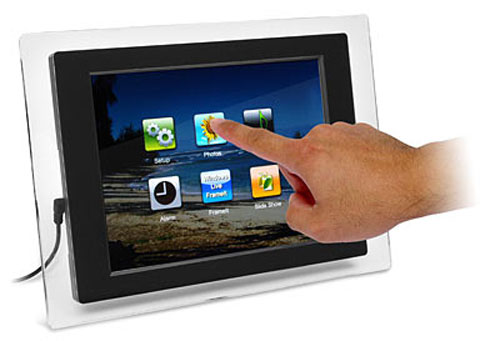
\includegraphics[width=0.1\textwidth]{touch} 
							\bigskip
							
						\end{itemize}
			\end{block}
					
		\end{frame}

	\section{Referencias Bibliogr\'aficas} 

		\begin{frame}\frametitle<presentation>{Referencias Bibliogr\'aficas}


			\begin{thebibliography}{10}

				\bibitem{lamport94}
					  Reto Meir, 
   					\emph{Professional Android Application Development}.
 					 Wiley Publishing, Inc,
  					  2009.

			\end{thebibliography}
		\end{frame}

\end{document}